\documentclass[11pt,a4paper]{article}

\usepackage{amsmath, amsthm, amssymb}
\usepackage{hyperref}
\usepackage{geometry}
\usepackage{graphicx}
\geometry{margin=2.5cm}

\newtheorem{proposition}{Proposition}
\newtheorem{lemma}{Lemma}
\newtheorem{remark}{Remark}
\newtheorem{definition}{Definition}

\title{Spectral Admissibility and Non-Abelian Mode Resilience
in the $Q_8$ Cayley Graph under Bounded Flux}
\author{Working note -- Cosmochrony programme}
\date{\today}

\begin{document}
  \maketitle

  \begin{abstract}
    We establish the first analytically tractable instance of the spectral admissibility
    programme outlined in the Cosmochrony framework.
    On the undirected Cayley graph of the quaternion group $Q_8$, with generators
    $S = \{\pm i, \pm j, \pm k\}$, the local bounded-flux constraint
    $|\partial_t \chi_v| \leq c_\chi$ induces a hierarchy of maximal admissible
    effective amplitudes across irreducible spectral sectors.

    In the linearised dispersion regime, the non-abelian irreducible sector
    admits a maximal effective amplitude larger than the nontrivial abelian sectors
    by a factor of $\sqrt{4/3} \approx 1.155$.
    Resolving explicitly the basis dependence in the degenerate $\rho_4$ eigenspace,
    we show that this advantage holds for the physically relevant effective amplitude
    $A_n = a_n \|\psi_n\|_\infty$, but not for the raw amplitude $a_n$.

    We then perform the weakly non-linear modal reduction of the discrete
    Dirac--Born--Infeld (DBI) Lagrangian and derive the first amplitude-dependent
    correction to the dispersion relation, governed by the quartic shape factor
    $\kappa_n = \sum_v \psi_n(v)^4$.
    When expressed in terms of the effective amplitude, this correction depends
    only on the Laplacian eigenvalue $\lambda_n$, leaving the spectral hierarchy
    unchanged.

    Finally, solving the one-mode DBI dynamics exactly on the $Q_8$ Cayley graph,
    we show that the admissibility envelope
    \[
      A_n^{\max} = \frac{c_\chi}{\sqrt{\lambda_n}}
    \]
    coincides with the exact saturation boundary of the DBI dynamics.
    The spectral hierarchy therefore remains structurally stable beyond the
    perturbative regime.

    This provides a minimal explicit demonstration that bounded substrate capacity
    can favour non-abelian relational modes purely through spectral admissibility,
    without invoking additional dynamical selection principles.

    We further extend the analysis to the binary icosahedral group $2I$,
    the largest finite subgroup of $\mathrm{SU}(2)$.
    Using the order-10 generating classes, the same admissibility envelope
    produces a four-level spectral hierarchy across the spin sectors of $2I$,
    with an admissibility contrast $\sqrt{14/9}$ between the most and least
    admissible non-trivial sectors.
    This provides the second explicit instance of the spectral admissibility
    programme along the chain
    \[
      Q_8 \subset 2I \subset \mathrm{SU}(2).
    \]

    More broadly, it suggests that non-abelian symmetry sectors may emerge
    as the dynamically most resilient components of the relational spectrum
    under bounded-flux constraints.
  \end{abstract}

  \section{Setting and Motivation}

    The Cosmochrony framework identifies the physical spectrum with the residue of two
    successive constraints acting on the relational operator $\mathcal{L}_\chi$:
    \begin{enumerate}
      \item \textbf{Topological discretisation}: the fibre structure of the non-injective
      projection $\Pi$ organises modes into discrete winding sectors.
      \item \textbf{Bounded-flux filtering}: the saturation bound
      $|\partial_t \chi| \leq c_\chi$ eliminates modes whose local evolution would
      exceed the substrate's relational capacity.
    \end{enumerate}
    The goal of this note is to make step~2 explicit and calculable on the simplest
    non-trivial finite graph encoding a quaternionic algebraic structure,
    as a minimal discrete proxy for $\mathrm{SU}(2)$-type sectors.

  \section{The $Q_8$ Cayley Graph}

    Let $Q_8 = \{{\pm 1, \pm i, \pm j, \pm k}\}$ denote the quaternion group of order~8.
    We define the undirected Cayley graph $\Gamma(Q_8, S)$ with generating set
    \begin{equation}
      S = \{\pm i, \pm j, \pm k\}.
    \end{equation}
    Since $S$ is closed under inversion ($s^{-1} \in S$ for all $s \in S$) and does
    not contain the identity, $\Gamma(Q_8, S)$ is a well-defined, connected, undirected,
    $6$-regular graph on $8$ vertices.

    \begin{remark}
      The choice $S = \{i, j, k\}$ without inverses would yield a directed graph with an
      asymmetric adjacency operator.
      For a self-adjoint Laplacian, the full symmetric set
      $S = \{\pm i, \pm j, \pm k\}$ is required.
      The resulting graph is $6$-regular, not $3$-regular.
    \end{remark}

    \subsection{Adjacency Operator and Graph Laplacian}

      The adjacency operator $A$ of $\Gamma(Q_8, S)$ acts on functions
      $f \colon Q_8 \to \mathbb{C}$ by
      \begin{equation}
        (Af)(g) = \sum_{s \in S} f(gs)
      = \sum_{s \in \{\pm i, \pm j, \pm k\}} f(gs).
      \end{equation}
      The combinatorial graph Laplacian is
      \begin{equation}
        \mathcal{L} = dI - A,
        \qquad
        d = |S| = 6,
      \end{equation}
      where $I$ is the identity on $\ell^2(Q_8)$.
      The eigenvalues of $\mathcal{L}$ are $\lambda = 6 - \mu$, where $\mu$ ranges over
      the eigenvalues of $A$.

  \section{Spectral Decomposition via Representation Theory}

    Since $Q_8$ is a finite group, $\ell^2(Q_8) \cong \mathbb{C}[Q_8]$ decomposes
    as a $Q_8$-module into irreducible representations.
    By the Peter--Weyl theorem for finite groups:
    \begin{equation}
      \mathbb{C}[Q_8] \cong \bigoplus_{\rho \in \widehat{Q_8}} V_\rho^{\oplus \dim \rho},
    \end{equation}
    where the sum runs over the five irreducible representations of $Q_8$.

    \subsection{Irreducible Representations of $Q_8$}

      $Q_8$ has five irreducible representations:
      \begin{center}
        \begin{tabular}{lcccc}
          \hline
          Label              & Dimension & $\rho(i)$ & $\rho(j)$ & $\rho(k)$ \\
          \hline
          $\rho_0$ (trivial) & 1         & $1$       & $1$       & $1$       \\
          $\rho_1$           & 1         & $1$       & $-1$      & $-1$      \\
          $\rho_2$           & 1         & $-1$      & $1$       & $-1$      \\
          $\rho_3$           & 1         & $-1$      & $-1$      & $1$       \\
          $\rho_4$ (quaternionic) & 2 &
          $\begin{pmatrix}
             i&0\\0&-i
          \end{pmatrix}$ &
          $\begin{pmatrix}
             0&1\\-1&0
          \end{pmatrix}$ &
          $\begin{pmatrix}
             0&i\\i&0
          \end{pmatrix}$ \\
          \hline
        \end{tabular}
      \end{center}
      The dimension check:
      $1^2 + 1^2 + 1^2 + 1^2 + 2^2 = 8 = |Q_8|$.

    \subsection{Eigenvalues of the Adjacency Operator}

      For any irreducible representation $\rho$, the adjacency operator acts as the
      scalar $\mu_\rho \cdot I_{V_\rho}$ on $V_\rho$.
      Since $S$ is a union of conjugacy classes of $Q_8$, the corresponding element
      of the group algebra is central, and Schur's lemma gives
      \begin{equation}
        \mu_\rho = \frac{1}{\dim \rho} \sum_{s \in S} \chi_\rho(s),
      \end{equation}
      where $\chi_\rho$ is the character of $\rho$.

      \paragraph{1D sectors.}
        For the trivial representation $\rho_0$, $\chi_{\rho_0}(s) = 1$ for all
        $s \in S$, so $\sum_{s \in S} \chi_{\rho_0}(s) = 6$ and
      \begin{equation}
        \mu_{\rho_0} = 6,
        \qquad
        \lambda_{\rho_0} = 6 - 6 = 0.
        \end{equation}
        For $\rho_1$, $\chi_{\rho_1}(\pm i) = 1$ and
        $\chi_{\rho_1}(\pm j) = \chi_{\rho_1}(\pm k) = -1$,
        so $\sum_{s \in S} \chi_{\rho_1}(s) = 2(1) + 4(-1) = -2$, giving
        $\mu_{\rho_1} = -2$ and $\lambda_{\rho_1} = 8$.
        By the symmetry of $Q_8$ under permutations of $\{i,j,k\}$,
        $\mu_{\rho_2} = \mu_{\rho_3} = -2$ and
        $\lambda_{\rho_2} = \lambda_{\rho_3} = 8$.

      \paragraph{2D sector.}
        For the quaternionic representation $\rho_4$, we compute the character at each
        generator.
        The matrices $\rho_4(i)$, $\rho_4(-i)$, $\rho_4(j)$, $\rho_4(-j)$,
        $\rho_4(k)$, $\rho_4(-k)$ each have trace zero.
        Thus $\sum_{s \in S} \chi_{\rho_4}(s) = 0$ and
      \begin{equation}
        \mu_{\rho_4} = 0,
        \qquad
        \lambda_{\rho_4} = 6.
        \end{equation}

  \subsection{Summary of the Spectrum}

    \begin{center}
      \begin{tabular}{lccc}
        \hline
        Sector                   & $\lambda_n$ & Multiplicity & Type                     \\
        \hline
        $\rho_0$                 & $0$         & $1$          & Trivial zero mode        \\
        $\rho_1, \rho_2, \rho_3$ & $8$         & $3$          & Nontrivial abelian       \\
        $\rho_4$                 & $6$         & $4$          & Non-abelian quaternionic \\
        \hline
      \end{tabular}
    \end{center}
    Total dimension: $1 + 3 + 4 = 8$.

  \section{Bounded-Flux Admissibility Condition}

  \subsection{Setup}

    Let the substrate field $\chi \colon Q_8 \times \mathbb{R} \to \mathbb{R}$ evolve
    on the graph, subject to the local bounded-flux constraint
    \begin{equation}
      \label{eq:flux-bound}
      |\partial_t \chi_v(t)| \leq c_\chi
      \qquad
      \forall v \in Q_8,
      \ \forall t.
    \end{equation}
    Consider a single-mode excitation
    \begin{equation}
      \chi_v(t) = a_n \psi_n(v) \cos(\omega_n t),
    \end{equation}
    where $\psi_n$ is an eigenmode of $\mathcal{L}$ with eigenvalue $\lambda_n$,
    normalised in $\ell^2(Q_8)$, and $a_n > 0$ is the mode amplitude.
    The time derivative at vertex $v$ is
    \begin{equation}
      \partial_t \chi_v(t) = -a_n \omega_n \psi_n(v) \sin(\omega_n t).
    \end{equation}
    The constraint~\eqref{eq:flux-bound} requires
    \begin{equation}
      |\omega_n| \cdot a_n \cdot |\psi_n(v)| \leq c_\chi
      \qquad
      \forall v \in Q_8.
    \end{equation}
    The binding constraint is at the vertex where $|\psi_n(v)|$ is maximal:
    \begin{equation}
      |\omega_n| \cdot a_n \cdot \|\psi_n\|_\infty \leq c_\chi.
    \end{equation}

  \subsection{Effective Amplitude and Admissibility Envelope}

    \begin{definition}
      The effective amplitude of a mode $(\psi_n, a_n)$ is
      \begin{equation}
        A_n := a_n \|\psi_n\|_\infty.
      \end{equation}
      A mode is dynamically admissible in the linearised regime if
      \begin{equation}
        \label{eq:admissibility}
        |\omega_n| \cdot A_n \leq c_\chi.
      \end{equation}
    \end{definition}

    In the linearised dispersion approximation, $\omega_n^2 \approx \lambda_n$, so the
    maximal admissible effective amplitude is
    \begin{equation}
      \label{eq:envelope}
      A_n^{\max} = \frac{c_\chi}{\sqrt{\lambda_n}}.
    \end{equation}
    This defines the admissibility envelope in the $(\lambda_n, A_n)$ plane.

    \begin{figure}[t]
      \centering
      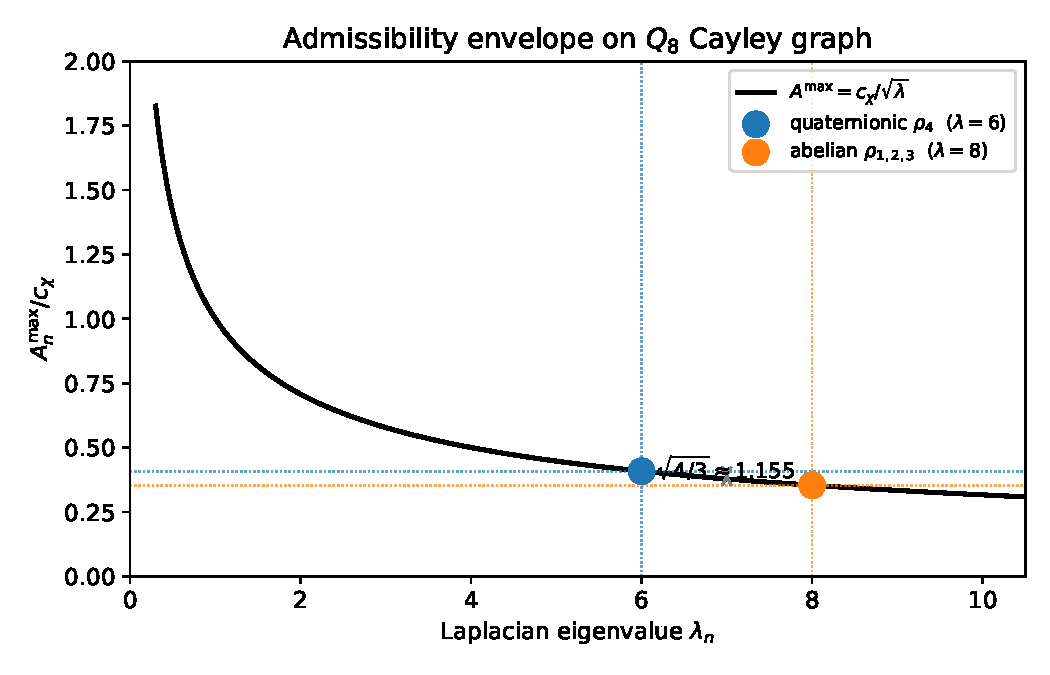
\includegraphics[width=0.82\textwidth]{fig1_Q8_admissibility}
      \caption{
        Admissibility envelope on the $Q_8$ Cayley graph with
        $S=\{\pm i,\pm j,\pm k\}$.
        The maximal effective amplitude
        $A_n^{\max}=c_\chi/\sqrt{\lambda_n}$
        is larger in the quaternionic non-abelian sector
        $\rho_4$ ($\lambda=6$) than in the non-trivial abelian sectors
        ($\lambda=8$), by the factor $\sqrt{4/3}$.
      }
      \label{fig:q8-admissibility}
    \end{figure}

    \begin{remark}
      The linearised dispersion $\omega_n^2 = \lambda_n$ is valid for
      $A_n \ll c_\chi / \sqrt{\lambda_n}$.
      The non-linear Born--Infeld correction modifies this relation near saturation and
      requires a modal reduction of the DBI action.
      The envelope~\eqref{eq:envelope} should therefore be understood first as the
      admissibility boundary in the weakly non-linear regime.
    \end{remark}

  \subsection{Explicit Eigenmodes in the $\rho_4$ Sector}
    \label{subsec:explicit-rho4}

    The non-abelian sector $\rho_4$ has multiplicity $4$ in $\ell^2(Q_8)$, so the
    quantity $\|\psi_n\|_\infty$ is not determined until an explicit basis of the
    eigenspace is chosen.
    A natural orthonormal basis is provided by the matrix coefficients of the
    quaternionic irreducible representation.

    For a finite group $G$ and an irreducible representation $\rho$, the standard
    Peter--Weyl basis of the corresponding isotypic component is given by
    \begin{equation}
      \psi_{uv}(g)
      =
      \sqrt{\frac{\dim \rho}{|G|}}\,\rho(g)_{uv},
      \qquad
      u,v \in \{1,\dots,\dim \rho\}.
    \end{equation}
    For $Q_8$ and $\rho_4$, this becomes
    \begin{equation}
      \psi_{uv}(g)
      =
      \frac{1}{2}\,\rho_4(g)_{uv},
      \qquad
      u,v \in \{1,2\},
    \end{equation}
    since $\dim \rho_4 = 2$ and $|Q_8| = 8$.

    Using the explicit matrices
    \begin{equation}
      \rho_4(1)=
      \begin{pmatrix}
        1 & 0 \\
        0 & 1
      \end{pmatrix},
      \qquad
      \rho_4(-1)=
      \begin{pmatrix}
        -1 & 0 \\
        0 & -1
      \end{pmatrix},
    \end{equation}
    \begin{equation}
      \rho_4(i)=
      \begin{pmatrix}
        i & 0 \\
        0 & -i
      \end{pmatrix},
      \qquad
      \rho_4(j)=
      \begin{pmatrix}
        0 & 1 \\
        -1 & 0
      \end{pmatrix},
      \qquad
      \rho_4(k)=
      \begin{pmatrix}
        0 & i \\
        i & 0
      \end{pmatrix},
    \end{equation}
    one finds that the diagonal modes $\psi_{11}, \psi_{22}$ are supported on
    $\{\pm 1, \pm i\}$, while the off-diagonal modes $\psi_{12}, \psi_{21}$ are
    supported on $\{\pm j, \pm k\}$.
    In all four cases,
    \begin{equation}
      |\psi_{uv}(g)| \in \left\{0,\frac{1}{2}\right\},
    \end{equation}
    hence
    \begin{equation}
      \|\psi_{uv}\|_\infty = \frac{1}{2},
      \qquad
      u,v \in \{1,2\}.
    \end{equation}

    For the one-dimensional nontrivial abelian sectors $\rho_1, \rho_2, \rho_3$,
    the normalised eigenmodes are the corresponding characters scaled by
    $|Q_8|^{-1/2}$.
    Since these characters take values in $\{\pm 1\}$, one has
    \begin{equation}
      \|\psi_{\rho_k}\|_\infty = \frac{1}{\sqrt{8}},
      \qquad
      k = 1,2,3.
    \end{equation}

  \subsection{Basis-Resolved Admissibility}

    \begin{proposition}[Basis-resolved admissibility on $Q_8$]
      \label{prop:basis-resolved}
      In the canonical Peter--Weyl basis of $\ell^2(Q_8)$, the maximal admissible
      effective amplitudes satisfy
      \begin{equation}
        A_{\rho_4}^{\max}
        =
        \frac{c_\chi}{\sqrt{6}}
        >
        \frac{c_\chi}{\sqrt{8}}
        =
        A_{\rho_k}^{\max},
        \qquad
        k=1,2,3,
      \end{equation}
      whereas the corresponding maximal raw amplitudes satisfy
      \begin{equation}
        a_{\rho_4}^{\max}
        =
        \frac{c_\chi}{\sqrt{6}\,\|\psi_{\rho_4}\|_\infty}
        =
        \frac{2}{\sqrt{6}}\,c_\chi
        \approx 0.816\,c_\chi,
      \end{equation}
      \begin{equation}
        a_{\rho_k}^{\max}
        =
        \frac{c_\chi}{\sqrt{8}\,\|\psi_{\rho_k}\|_\infty}
        =
        c_\chi,
        \qquad
        k=1,2,3.
      \end{equation}
      Thus the non-abelian sector is favoured in effective amplitude, but not in raw
      amplitude.
    \end{proposition}

    \begin{proof}
      The effective-amplitude statement follows from
      $A_n^{\max} = c_\chi/\sqrt{\lambda_n}$ together with
      $\lambda_{\rho_4} = 6$ and $\lambda_{\rho_k} = 8$.
      The raw-amplitude statement follows from
      $a_n^{\max} = A_n^{\max}/\|\psi_n\|_\infty$, using
      $\|\psi_{\rho_4}\|_\infty = 1/2$ and
      $\|\psi_{\rho_k}\|_\infty = 1/\sqrt{8}$.
    \end{proof}

  \subsection{Weakly Non-linear Modal DBI Reduction}
    \label{subsec:weakly-nonlinear-dbi}

    To incorporate the first Born--Infeld correction, consider the discrete DBI Lagrangian
    \begin{equation}
      \label{eq:dbi-lagrangian}
      L
      =
      -c_\chi^2 \sum_v \sqrt{1 - \dot{\chi}_v^2/c_\chi^2}
      - \tfrac{1}{2} \sum_{v,w} \chi_v \mathcal{L}_{vw} \chi_w.
    \end{equation}
    For a single eigenmode,
    \begin{equation}
      \chi_v(t) = q(t)\psi_n(v),
    \end{equation}
    with $\mathcal{L}\psi_n = \lambda_n \psi_n$ and $\|\psi_n\|_2 = 1$, this reduces to
    the exact one-mode Lagrangian
    \begin{equation}
      \label{eq:exact-mode-lagrangian}
      L_n[q]
      =
      -c_\chi^2 \sum_v \sqrt{1 - \psi_n(v)^2 \dot{q}^{\,2}/c_\chi^2}
      - \tfrac{1}{2}\lambda_n q^2.
    \end{equation}

    Expanding the square root for $|\dot{q}| \ll c_\chi$ gives
    \begin{equation}
      \label{eq:mode-lagrangian-expansion}
      L_n[q]
      =
      \mathrm{const}
      + \tfrac{1}{2}\dot{q}^{\,2}
      + \frac{\kappa_n}{8c_\chi^2}\dot{q}^{\,4}
      - \tfrac{1}{2}\lambda_n q^2
      + \mathcal{O}(c_\chi^{-4}),
    \end{equation}
    where
    \begin{equation}
      \label{eq:kappa-def}
      \kappa_n := \sum_v \psi_n(v)^4.
    \end{equation}
    The corresponding Euler--Lagrange equation is
    \begin{equation}
      \label{eq:weakly-nonlinear-mode-equation}
      \left(
        1 + \frac{3\kappa_n}{2c_\chi^2}\dot{q}^{\,2}
      \right)\ddot{q}
      + \lambda_n q
      = 0.
    \end{equation}

    Using the harmonic-balance ansatz
    \begin{equation}
      q(t) \approx a_n \cos(\omega_n t),
    \end{equation}
    and keeping only the fundamental harmonic, one obtains the first
    amplitude-dependent correction
    \begin{equation}
      \label{eq:omega-shift-square}
      \omega_n^2(a_n)
      \approx
      \lambda_n
      \left(
        1 - \frac{3\kappa_n\lambda_n a_n^2}{8c_\chi^2}
      \right),
    \end{equation}
    or equivalently
    \begin{equation}
      \label{eq:omega-shift}
      \omega_n(a_n)
      \approx
      \sqrt{\lambda_n}
      \left(
        1 - \frac{3\kappa_n\lambda_n a_n^2}{16c_\chi^2}
      \right).
    \end{equation}
    The DBI correction is therefore a softening non-linearity.

    In the canonical $Q_8$ basis, the quartic shape factor is explicit.
    For the one-dimensional nontrivial abelian sectors,
    \begin{equation}
      \label{eq:kappa-abelian}
      \kappa_{\rho_k}
      =
      \sum_{v \in Q_8} \left(\frac{1}{\sqrt{8}}\right)^4
      =
      \frac{1}{8},
      \qquad
      k = 1,2,3.
    \end{equation}
    For each canonical basis vector in the $\rho_4$ sector,
    \begin{equation}
      \label{eq:kappa-nonabelian}
      \kappa_{\rho_4}
      =
      4 \left(\frac{1}{2}\right)^4
      =
      \frac{1}{4}.
    \end{equation}

    However, rewriting the correction in terms of the effective amplitude
    $A_n = a_n\|\psi_n\|_\infty$ gives
    \begin{equation}
      \label{eq:omega-shift-effective}
      \omega_n^2(A_n)
      \approx
      \lambda_n
      \left(
        1
        - \frac{3\lambda_n A_n^2}{8c_\chi^2}
        \frac{\kappa_n}{\|\psi_n\|_\infty^2}
      \right).
    \end{equation}
    In the canonical $Q_8$ basis,
    \begin{equation}
      \frac{\kappa_{\rho_k}}{\|\psi_{\rho_k}\|_\infty^2}
      =
      \frac{(1/8)}{(1/\sqrt{8})^2}
      =
      1,
      \qquad
      \frac{\kappa_{\rho_4}}{\|\psi_{\rho_4}\|_\infty^2}
      =
      \frac{(1/4)}{(1/2)^2}
      =
      1.
    \end{equation}
    Therefore
    \begin{equation}
      \label{eq:omega-shift-effective-q8}
      \omega_n^2(A_n)
      \approx
      \lambda_n
      \left(
        1 - \frac{3\lambda_n A_n^2}{8c_\chi^2}
      \right)
    \end{equation}
    in both the nontrivial abelian and non-abelian sectors.

    \begin{figure}[t]
      \centering
      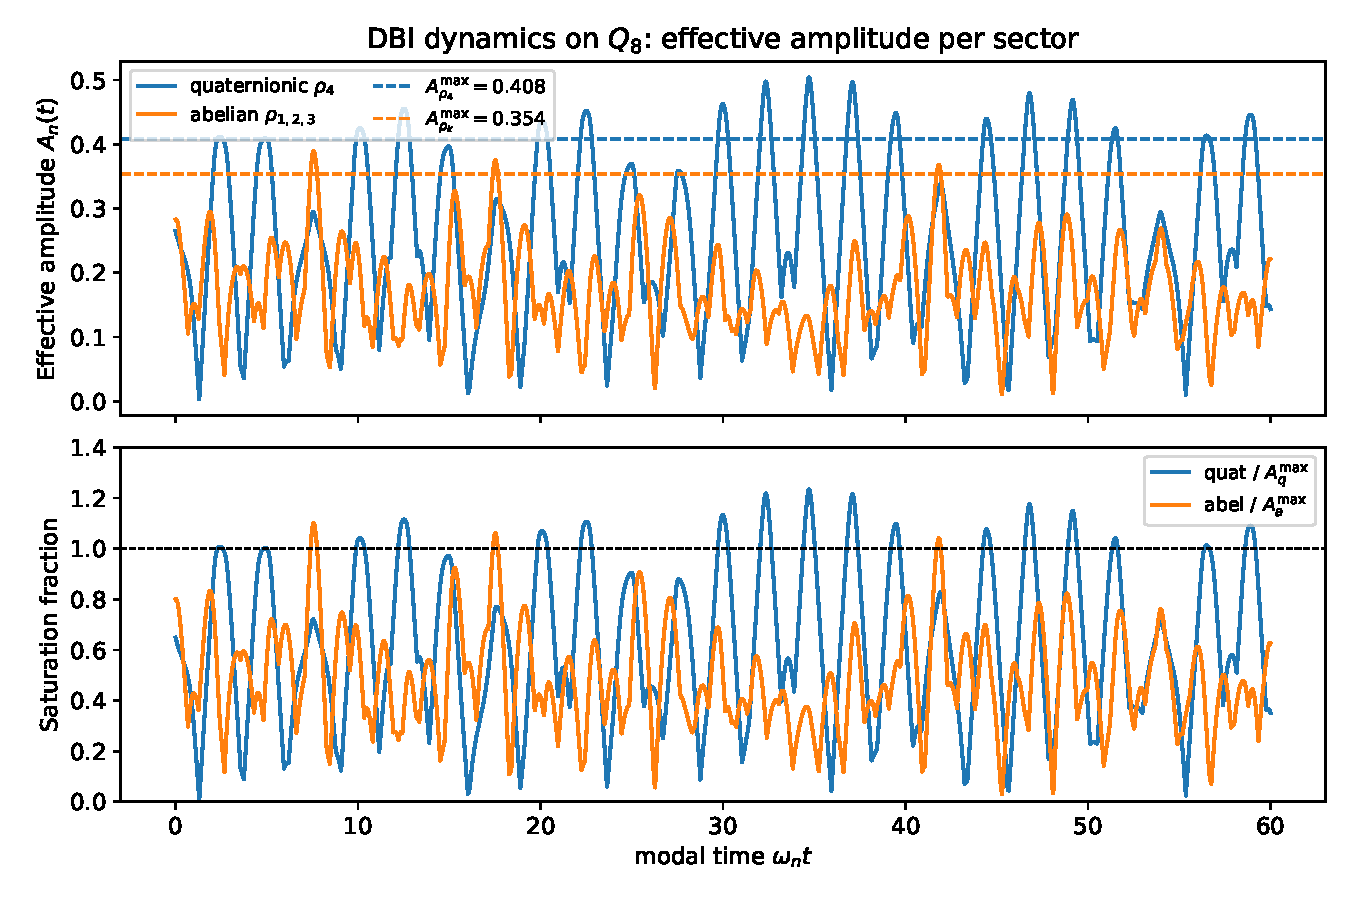
\includegraphics[width=0.9\textwidth]{fig2_Q8_DBI_dynamics}
      \caption{
        One-mode DBI dynamics on the $Q_8$ Cayley graph.
        Top: effective amplitudes in the quaternionic and abelian sectors.
        Bottom: corresponding saturation fractions relative to the exact
        admissibility bounds.
        The horizontal axis denotes the evolution parameter of the reduced
        modal dynamics.
        The quaternionic sector retains the largest admissible window,
        consistent with the spectral hierarchy derived from the bounded-flux
        constraint.
      }
      \label{fig:q8-dbi-dynamics}
    \end{figure}

    At fixed effective amplitude, the non-abelian sector thus remains less penalised
    by the weakly non-linear DBI correction, solely because $\lambda_{\rho_4}=6$
    is smaller than $\lambda_{\rho_k}=8$.

  \subsection{Non-perturbative DBI Envelope}
    \label{subsec:nonperturbative-dbi}

    The weakly non-linear reduction derived in
    Section~\ref{subsec:weakly-nonlinear-dbi} provides the leading
    amplitude correction to the dispersion relation.
    However, the discrete Dirac--Born--Infeld dynamics allows the
    single-mode problem to be solved exactly on the $Q_8$ Cayley graph.

    Consider again a single eigenmode
    \[
      \chi_v(t) = q(t)\psi_n(v),
    \]
    with $\mathcal{L}\psi_n = \lambda_n \psi_n$ and $\|\psi_n\|_2=1$.
    Substituting this ansatz into the DBI Lagrangian
    Eq.~\eqref{eq:dbi-lagrangian} gives the exact one-mode Lagrangian
    \begin{equation}
      L_n[q]
      =
      -c_\chi^2
      \sum_{v\in Q_8}
      \sqrt{1-\frac{\psi_n(v)^2\dot q^{\,2}}{c_\chi^2}}
      -
      \frac12\lambda_n q^2 .
    \end{equation}

    \subsubsection*{Abelian sectors}

      For the nontrivial abelian representations $\rho_1,\rho_2,\rho_3$,
      the normalized eigenmodes satisfy
      \[
        |\psi_n(v)| = \frac{1}{\sqrt{8}}
        \qquad
        \forall v\in Q_8 .
      \]
      The Lagrangian therefore becomes
      \begin{equation}
        L
        =
        -8c_\chi^2
        \sqrt{1-\frac{\dot q^{\,2}}{8c_\chi^2}}
        -
        \frac12\lambda_n q^2 .
      \end{equation}

    \subsubsection*{Non-abelian sector}

      For the quaternionic sector $\rho_4$ in the canonical basis,
      the eigenmodes satisfy
      \[
        |\psi_n(v)| =
        \begin{cases}
          \frac12 & \text{on four vertices}, \\
          0 & \text{on four vertices}.
        \end{cases}
      \]
      The DBI sum therefore reduces to
      \begin{equation}
        L
        =
        -4c_\chi^2
        \sqrt{1-\frac{\dot q^{\,2}}{4c_\chi^2}}
        -4c_\chi^2
        -
        \frac12\lambda_n q^2 .
      \end{equation}
      The constant term does not affect the dynamics, and the effective
      Lagrangian becomes
      \begin{equation}
        L
        =
        -4c_\chi^2
        \sqrt{1-\frac{\dot q^{\,2}}{4c_\chi^2}}
        -
        \frac12\lambda_n q^2 .
      \end{equation}

    \subsubsection*{Energy conservation}

      Since the Lagrangian is time independent, the corresponding Hamiltonian
      is conserved.
      One obtains
      \begin{equation}
        E
        =
        4c_\chi^2
        \frac{1}{\sqrt{1-\frac{\dot q^{\,2}}{4c_\chi^2}}}
        +
        \frac12\lambda_n q^2 .
      \end{equation}
      At the turning points $\dot q=0$, where $q=\pm a_n$, the energy becomes
      \begin{equation}
        E
        =
        4c_\chi^2
        +
        \frac12\lambda_n a_n^2 ,
      \end{equation}
      where $a_n$ denotes the raw oscillation amplitude of the modal coordinate.

    \subsubsection*{Velocity bound}

      The DBI square root imposes the kinematic bound
      \begin{equation}
        |\dot q| < 2c_\chi .
      \end{equation}
      Expressed in terms of the field variable,
      \[
        \chi_v = q\psi_n(v),
      \]
      this corresponds exactly to the local flux constraint
      \[
        |\partial_t \chi_v| \le c_\chi .
      \]

    \subsubsection*{Amplitude bound}

      The turning point occurs when the maximal vertex saturates the flux bound,
      \[
        |\partial_t\chi_v|
        =
        |\dot q|\,|\psi_n(v)|
        =
        c_\chi .
      \]
      Since $\|\psi_n\|_\infty$ is the maximal value of $|\psi_n(v)|$, this gives
      \begin{equation}
        a_n^{\max}
        =
        \frac{c_\chi}{\|\psi_n\|_\infty\sqrt{\lambda_n}} .
      \end{equation}
      The corresponding effective amplitude
      \[
        A_n = a_n\|\psi_n\|_\infty
      \]
      therefore satisfies
      \begin{equation}
        A_n^{\max}
        =
        \frac{c_\chi}{\sqrt{\lambda_n}} .
      \end{equation}

    \subsubsection*{Exact admissibility envelope}

      We thus obtain the non-perturbative result
      \begin{equation}
        A_n^{\max}
        =
        \frac{c_\chi}{\sqrt{\lambda_n}},
      \end{equation}
      which coincides exactly with the admissibility envelope derived from the
      linear bounded-flux argument.

      The weakly non-linear correction therefore does not modify the
      location of the admissibility boundary.
      Instead, the DBI dynamics smoothly interpolates between the linear regime
      and a velocity-saturated regime as the amplitude approaches the bound.

      This shows that the spectral admissibility envelope identified above is not
      merely a linear approximation but the exact saturation boundary for the
      single-mode DBI dynamics on the $Q_8$ Cayley graph.

  \section{Admissibility Hierarchy on the $Q_8$ Cayley Graph}

  \begin{proposition}[Spectral admissibility hierarchy on $Q_8$]
    \label{prop:main}
    In the undirected Cayley graph $\Gamma(Q_8, \{\pm i, \pm j, \pm k\})$,
    under the local bounded-flux constraint~\eqref{eq:flux-bound} and linearised
    dispersion, the maximal admissible effective amplitude satisfies
    \begin{equation}
      A^{\max}_{\rho_4} = \frac{c_\chi}{\sqrt{6}}
      >
      \frac{c_\chi}{\sqrt{8}}
      = A^{\max}_{\rho_k},
      \qquad
      k = 1,2,3.
    \end{equation}
    The non-abelian sector $\rho_4$ occupies a strictly larger admissible region in the
    space of effective mode amplitudes than any nontrivial abelian sector, by a factor
    \begin{equation}
      \frac{A^{\max}_{\rho_4}}{A^{\max}_{\rho_k}}
      =
      \sqrt{\frac{8}{6}}
      =
      \sqrt{\frac{4}{3}}
      \approx 1.155.
    \end{equation}
  \end{proposition}

  \begin{proof}
    Direct substitution of $\lambda_{\rho_4} = 6$ and $\lambda_{\rho_k} = 8$
    into the admissibility envelope~\eqref{eq:envelope}.
  \end{proof}

  \begin{remark}
    The trivial sector $\rho_0$ has $\lambda = 0$ and thus formally unbounded $A^{\max}$.
    It corresponds to the uniform zero mode of the connected graph.
    In the present analysis it is factored out, since we are interested only in
    non-trivial excitations above the connected background.
  \end{remark}

  Proposition~\ref{prop:main}, together with
  Proposition~\ref{prop:basis-resolved}, establishes that, at fixed substrate capacity
  $c_\chi$, the non-abelian irreducible sector of the quaternion Cayley graph sustains
  a larger local effective amplitude before violating the bounded-flux constraint,
  even though its raw amplitude bound is lower than that of the nontrivial abelian
  sectors.

  In the language of the Cosmochrony programme:
  \begin{itemize}
    \item The admissibility envelope $A_n^{\max} = c_\chi / \sqrt{\lambda_n}$ defines a
    geometry of exclusion in the space of relational modes.
    Modes above the envelope are dynamically inadmissible.
    \item The non-abelian sector $\rho_4$ lies below this envelope for a larger
    range of effective amplitudes than the nontrivial abelian sectors
    $\rho_1, \rho_2, \rho_3$.
    The bounded-flux constraint is therefore less restrictive for non-abelian modes,
    enlarging their admissible window by a factor of $\sqrt{4/3}$.
    \item This advantage is a statement about the physically relevant local variable
    $A_n = a_n \|\psi_n\|_\infty$, not about the raw amplitude $a_n$.
    \item In the canonical basis, the weakly non-linear DBI correction again favours
    the non-abelian sector through its smaller eigenvalue.
    \item The exact one-mode DBI analysis shows that the same envelope
    $A_n^{\max} = c_\chi/\sqrt{\lambda_n}$ remains the true saturation boundary.
  \end{itemize}

  \begin{remark}[Real field and complex eigenmodes]
      The substrate field $\chi$ is taken real-valued.
      The natural eigenmodes of the 2D sector are matrix coefficients of $\rho_4$,
      which are complex-valued.
      One may either work in $\ell^2(Q_8,\mathbb{C})$ and take real and imaginary parts to
      obtain real eigenmodes, or directly choose a real basis for each eigenspace.
      The local admissibility criterion is intrinsically defined, but its expression in
      terms of $(a_n,\psi_n)$ depends on the chosen basis within a degenerate eigenspace
      through $\|\psi_n\|_\infty$.
      This basis dependence is resolved explicitly in
      Section~\ref{subsec:explicit-rho4}.
  \end{remark}

  \section{Synthesis: Spectral Filtering by Bounded Flux}

  The analysis performed in this note identifies the effective amplitude
  \[
    A_n = a_n \|\psi_n\|_\infty
  \]
  as the physically relevant variable controlling the saturation of the
  substrate.

  \subsection{Local Flux Constraint as a Spectral Filter}

    The bounded-flux condition
    \[
      |\partial_t \chi_v| \le c_\chi
    \]
    acts locally on each vertex of the relational substrate.

    For a single eigenmode
    \[
      \chi_v(t) = a_n \psi_n(v) \cos(\omega_n t),
    \]
    the constraint becomes
    \[
      |\omega_n|\,a_n\,\|\psi_n\|_\infty \le c_\chi.
    \]

    Introducing the effective amplitude
    \[
      A_n = a_n \|\psi_n\|_\infty
    \]
    yields the admissibility envelope
    \[
      A_n^{\max} = \frac{c_\chi}{\sqrt{\lambda_n}}.
    \]

    A key consequence is that localisation of the mode does not alter the
    admissibility bound itself.
    Localisation only determines how the raw amplitude $a_n$ translates into
    a local flux impact on the substrate.
    The selection mechanism is therefore governed by the spectral
    eigenvalue $\lambda_n$.

  \subsection{DBI Softening as Dynamical Spectral Filtering}

    In the weakly non-linear regime the discrete Dirac--Born--Infeld dynamics
    produces an amplitude-dependent frequency
    \[
      \omega_n^2(A_n)
      \approx
      \lambda_n
      \left(
        1 -
        \frac{3\lambda_n A_n^2}{8c_\chi^2}
      \right).
    \]

    This simplified expression follows from the identity
    \[
      \frac{\kappa_n}{\|\psi_n\|_\infty^2}=1
    \]
    which holds for all non-trivial sectors of the $Q_8$ Cayley graph.

    The non-linear correction therefore depends only on the Laplacian
    eigenvalue.
    Modes with larger $\lambda_n$ undergo stronger softening as the
    effective amplitude increases.

    The relational substrate thus behaves as a dynamical low-pass spectral
    filter.

  \subsection{Conceptual Interpretation}

    The mechanism uncovered in this toy model can be summarised as
    \[
      \text{sub\-strate capacity}
      \;\rightarrow\;
      \text{spectral admissibility}
      \;\rightarrow\;
      \text{nonlinear filtering}
      \;\rightarrow\;
      \text{surviving sectors}.
    \]

    On the $Q_8$ Cayley graph the smallest non-trivial eigenvalue
    \[
      \lambda_{\rho_4}=6
    \]
    belongs to the quaternionic non-abelian sector.
    This sector therefore possesses the largest admissible amplitude window
    and is the least affected by DBI softening.

    The non-perturbative DBI reduction derived in
    Section~\ref{subsec:nonperturbative-dbi} shows that the admissibility
    envelope
    \[
      A_n^{\max} = \frac{c_\chi}{\sqrt{\lambda_n}}
    \]
    is not merely a linear approximation.
    It coincides with the exact saturation boundary of the one-mode
    DBI dynamics on the $Q_8$ Cayley graph.

    The bounded relational capacity of the substrate therefore acts
    not merely as a spectral cut-off but as a dynamical selector,
    favouring the most resilient spectral sectors.

  \subsection{Beyond the $Q_8$ Toy Model}

    The identity
    \[
      \frac{\kappa_n}{\|\psi_n\|_\infty^2}=1
    \]
    is a special feature of the small and highly symmetric $Q_8$ graph.

    On larger graphs this ratio will generally depend on the structure of
    the eigenmodes.
    The non-linear DBI correction may therefore amplify the spectral
    selection mechanism rather than acting uniformly across sectors.

  \section{Structural Origin of the Admissibility Hierarchy and the SU(2) Emergence Thread}
  \label{sec:step4}

  \subsection{The ratio $\sqrt{4/3}$ is not accidental}
    \label{sec:step4-origin}

    The admissibility hierarchy established in Proposition~\ref{prop:main},
    \begin{equation}
      \frac{A^{\max}_{\rho_4}}{A^{\max}_{\rho_k}}
      = \sqrt{\frac{8}{6}} = \sqrt{\frac{4}{3}} \approx 1.155,
      \label{eq:ratio}
    \end{equation}
    has a precise internal origin in the $Q_8$ Cayley spectrum.
    It originates entirely from the Laplacian eigenvalues
    $\lambda_{\rho_4} = 6$ and $\lambda_{\rho_k} = 8$.
    The ratio $8/6$ is in turn fixed by the adjacency eigenvalues
    $\mu_{\rho_k} = -2$ and $\mu_{\rho_4} = 0$ through $\lambda = d - \mu$ with $d = 6$.

    The central observation is that $\mu_{\rho_4} = 0$.
    The quaternionic sector lies exactly at the centre of the adjacency spectrum.
    This is a structural consequence of the character theory of $Q_8$,
    not a numerical coincidence.

  \subsection{Why $\mu_{\rho_4} = 0$: character-theoretic argument}
    \label{sec:step4-character}

    For any Cayley graph on a finite group $G$ with symmetric generating set $S$,
    Schur's lemma gives the adjacency eigenvalue in the irreducible sector $\rho$ as
    \begin{equation}
      \mu_\rho = \frac{1}{\dim \rho} \sum_{s \in S} \chi_\rho(s).
      \label{eq:mu-character}
    \end{equation}
    For the quaternionic representation $\rho_4$ of $Q_8$, the generating set
    $S = \{\pm i, \pm j, \pm k\}$ maps to the matrices
    \begin{equation}
      \rho_4({\pm i}) = \pm\begin{pmatrix}
                             i & 0 \\ 0 & -i
      \end{pmatrix},
      \quad
      \rho_4({\pm j}) = \pm\begin{pmatrix}
                             0 & 1 \\ -1 & 0
      \end{pmatrix},
      \quad
      \rho_4({\pm k}) = \pm\begin{pmatrix}
                             0 & i \\ i & 0
      \end{pmatrix}.
    \end{equation}
    All six generator matrices are traceless.
    Therefore
    \begin{equation}
      \chi_{\rho_4}(s) = \mathrm{tr}(\rho_4(s)) = 0
      \qquad
      \forall\, s \in S,
      \label{eq:vanishing-character}
    \end{equation}
    and the character sum in Eq.~\eqref{eq:mu-character} vanishes identically,
    giving $\mu_{\rho_4} = 0$.

    This is a structural property.
    The generators of $Q_8$ map to traceless matrices under $\rho_4$
    because $Q_8$ is generated by the unit quaternions $i,j,k$,
    whose matrix images are exactly the imaginary units of $\mathrm{SU}(2)$.

  \subsection{$Q_8$ as the minimal discrete encoding of spin}
    \label{sec:step4-spin}

    The connection between $Q_8$ and spin is not coincidental but topological.
    The simply-connected double cover of $SO(3)$ is $\mathrm{SU}(2)$,
    which is topologically the three-sphere $S^3$:
    \begin{equation}
      \mathrm{SU}(2)
      \cong
      \big\{a_0 I + i a_1 \sigma_x + i a_2 \sigma_y + i a_3 \sigma_z
      \;:\;
      a_0^2 + a_1^2 + a_2^2 + a_3^2 = 1\big\}
      \cong S^3.
      \label{eq:SU2-S3}
    \end{equation}

    The group $Q_8 = \{\pm 1, \pm i, \pm j, \pm k\}$ is the smallest
    non-abelian subgroup of the unit quaternions, hence the smallest
    non-abelian subgroup of $\mathrm{SU}(2)$.
    Its elements encode the minimal subgroup structure compatible with spinorial
    $\mathrm{SU}(2)$ geometry.

  \subsection{Connection with the $S^3$ spectral invariant $\lambda_2/\lambda_1 = 8/3$}
    \label{sec:step4-S3}

    On the three-sphere $S^3$, the Laplacian eigenvalues are
    $\lambda_\ell = \ell(\ell + 2)$ with multiplicity $(\ell+1)^2$, giving
    \begin{equation}
      \ell = 0:\;\lambda_0 = 0,
      \qquad
      \ell = 1:\;\lambda_1 = 3,
      \qquad
      \ell = 2:\;\lambda_2 = 8,
      \qquad
      \ell = 3:\;\lambda_3 = 15.
    \end{equation}
    The fundamental spectral ratio of $S^3$ is
    \begin{equation}
      \frac{\lambda_2}{\lambda_1}\bigg|_{S^3} = \frac{8}{3}.
      \label{eq:S3-ratio}
    \end{equation}
    This ratio is the primary spectral invariant used elsewhere in the
    Cosmochrony programme to characterise the $S^3$ geometry from the
    relational spectrum~\cite{Spectral121}.

    The ratio from the present $Q_8$ calculation,
    \begin{equation}
      \frac{\lambda_{\rho_k}}{\lambda_{\rho_4}} = \frac{8}{6} = \frac{4}{3},
    \end{equation}
    is related heuristically to the $S^3$ ratio by
    \begin{equation}
      \frac{\lambda_{\rho_k}}{\lambda_{\rho_4}}
      = \frac{1}{2}\cdot\frac{\lambda_2}{\lambda_1}\bigg|_{S^3}.
      \label{eq:ratio-relation}
    \end{equation}

  \subsection{The SU(2) emergence programme}
    \label{sec:step4-programme}

    The $Q_8$ result motivates a systematic programme toward $\mathrm{SU}(2)$
    emergence via spectral admissibility.
    The key chain of inclusions is
    \begin{equation}
      Q_8 \subset 2I \subset \mathrm{SU}(2),
      \label{eq:inclusion-chain}
    \end{equation}
    where $2I$ is the binary icosahedral group of order $120$.

    The asymptotic step is provided by the Ramanujan graphs of
    Lubotzky, Phillips, and Sarnak~\cite{LPS1988}, which are Cayley graphs of
    $\mathrm{SL}(2,\mathbb{F}_p)$ designed to approximate $S^3$ with near-optimal
    spectral gap.

  \subsection{Physical interpretation}
    \label{sec:step4-physics}

    The non-abelian quaternionic sector has zero net correlation with the
    generators of the graph, $\mu_{\rho_4} = 0$.
    This neutrality is the source of its resilience.
    The bounded-flux constraint imposes less penalty on modes that do not couple
    positively or negatively to the relational connectivity.

    The mechanism is therefore a structural consequence of the embedding
    $Q_8 \hookrightarrow \mathrm{SU}(2)$ together with bounded substrate capacity:
    \begin{equation}
      \text{bounded relational capacity}
      \;\Longrightarrow\;
      \text{non-abelian sector resilience}.
    \end{equation}

  \section{Spectral Admissibility on the Binary Icosahedral Group $2I$}
  \label{sec:step5}

  \subsection{The group $2I$ and its place in the programme}
    \label{sec:step5-intro}

    The binary icosahedral group $2I$ is the double cover of the icosahedral
    rotation group $A_5 \cong \mathrm{PSL}(2,\mathbb{F}_5)$, and has order
    $|2I| = 120$.
    It is the largest finite subgroup of $\mathrm{SU}(2)$ and sits in the
    inclusion chain
    \begin{equation}
      Q_8 \subset 2I \subset \mathrm{SU}(2),
      \label{eq:chain}
    \end{equation}
    making it the natural next test case for the spectral admissibility
    programme.

    The irreducible representations of $2I$ are labelled by spin and have
    dimensions matching the low-spin content of $\mathrm{SU}(2)$:
    \begin{equation}
      \underbrace{1}_{\text{spin }0},\quad
      \underbrace{2,\,2'}_{\text{spin }\tfrac{1}{2}},\quad
      \underbrace{3,\,3'}_{\text{spin }1},\quad
      \underbrace{4,\,4'}_{\text{spin }\tfrac{3}{2}},\quad
      \underbrace{5}_{\text{spin }2},\quad
      \underbrace{6}_{\text{spin }\tfrac{5}{2}}.
      \label{eq:2I-irreps}
    \end{equation}
    Of these nine irreps, six are spin-type in the sense that they arise from
    restrictions of $\mathrm{SU}(2)$ representations.

  \subsection{Conjugacy classes and character table}
    \label{sec:step5-chars}

    The group $2I$ has nine conjugacy classes, enumerated by element order:
    \begin{center}
      \begin{tabular}{llcl}
        \hline
        Class & Order & Size & Notation                      \\
        \hline
        $1a$  & 1     & 1    & identity                      \\
        $2a$  & 2     & 1    & central element $-\mathbf{1}$ \\
        $3a$  & 3     & 20   &                               \\
        $4a$  & 4     & 30   &                               \\
        $5a$  & 5     & 12   &                               \\
        $5b$  & 5     & 12   & algebraic conjugate of $5a$   \\
        $6a$  & 6     & 20   &                               \\
        $10a$ & 10    & 12   &                               \\
        $10b$ & 10    & 12   & algebraic conjugate of $10a$  \\
        \hline
      \end{tabular}
    \end{center}
    The class sizes satisfy
    \[
      1+1+20+30+12+12+20+12+12 = 120.
    \]

    Writing $\varphi = (1+\sqrt{5})/2$ and
    $\bar\varphi = 1/\varphi = \varphi - 1 = (\sqrt{5}-1)/2$, the character
    values of the spin-type irreps are
    \begin{equation}
      \renewcommand{\arraystretch}{1.3}
      \begin{array}{l|rrrrrrrrr}
        & 1a & 2a & 3a & 4a & 5a & 5b & 6a & 10a & 10b \\
        \hline
        \chi_1 & 1 &  1 &  1 &  1 &  1 &  1 &  1 &  1 &  1 \\
        \chi_2 & 2 & -2 & -1 &  0 & \bar\varphi & -\varphi & 1 & \varphi & -\bar\varphi \\
        \chi_3 & 3 &  3 &  0 & -1 & \varphi & -\bar\varphi & 0 & -\bar\varphi & \varphi \\
        \chi_4 & 4 & -4 &  1 &  0 & -1 & -1 & -1 & 1 & 1 \\
        \chi_5 & 5 &  5 & -1 &  1 &  0 &  0 & -1 & 0 & 0 \\
        \chi_6 & 6 & -6 &  0 &  0 &  1 &  1 &  0 & -1 & -1
      \end{array}
      \label{eq:CT-2I}
    \end{equation}

  \subsection{Generating set: order-10 elements}
    \label{sec:step5-genset}

    A natural generating set for the comparison with $Q_8$ is the union of
    the two order-10 conjugacy classes,
    \begin{equation}
      S = 10a \cup 10b,
      \qquad
      |S| = 24.
      \label{eq:S-2I}
    \end{equation}
    This choice is canonical because it is inversion-symmetric, spinorially
    analogous to the $Q_8$ generating set, and generates $2I$.

  \subsection{Adjacency eigenvalues and spectral hierarchy}
    \label{sec:step5-spectrum}

    For a generating set that is a union of conjugacy classes, the adjacency
    eigenvalue in the irreducible sector $\rho$ is
    \begin{equation}
      \mu_\rho
      = \frac{1}{\dim\rho}
      \sum_{C \subseteq S} |C|\,\chi_\rho(C).
      \label{eq:mu-formula-2I}
    \end{equation}
    For $S = 10a \cup 10b$, with both classes of size $12$, this gives
    \begin{equation}
      \renewcommand{\arraystretch}{1.4}
      \begin{array}{l|ccc}
        \text{Sector} &
        \mu_\rho &
        \lambda_\rho = 24 - \mu_\rho &
        A^{\max}_\rho = c_\chi/\sqrt{\lambda_\rho} \\
        \hline
        \chi_1\;(\text{trivial}) & 24 & 0  & \infty \\
        \chi_2\;(\text{spin-}{\tfrac{1}{2}}) & 6  & 18 & c_\chi/\sqrt{18} \\
        \chi_3\;(\text{spin-}1) & 4  & 20 & c_\chi/\sqrt{20} \\
        \chi_4\;(\text{spin-}{\tfrac{3}{2}}) & 6  & 18 & c_\chi/\sqrt{18} \\
        \chi_5\;(\text{spin-}2) & 0  & 24 & c_\chi/\sqrt{24} \\
        \chi_6\;(\text{spin-}{\tfrac{5}{2}}) & -4 & 28 & c_\chi/\sqrt{28}
      \end{array}
      \label{eq:2I-spectrum}
    \end{equation}

    The spectral ordering of the non-trivial spin-type sectors is therefore
    \begin{equation}
      \lambda_{1/2} = \lambda_{3/2} = 18
      < \lambda_1 = 20
      < \lambda_2 = 24
      < \lambda_{5/2} = 28.
      \label{eq:2I-ordering}
    \end{equation}

  \subsection{Algebraic origin: the golden ratio identity}
    \label{sec:step5-golden}

    For the spin-$\tfrac{1}{2}$ sector,
    \begin{equation}
      \mu_2
      = \frac{1}{2}\bigl(12\,\chi_2(10a) + 12\,\chi_2(10b)\bigr)
      = 6\bigl(\chi_2(10a)+\chi_2(10b)\bigr).
      \label{eq:mu2-computation}
    \end{equation}
    Using
    \begin{equation}
      \chi_2(10a)+\chi_2(10b)
      = \varphi + (-\bar\varphi)
      = \varphi - \bar\varphi
      = 1,
      \label{eq:golden-identity}
    \end{equation}
    we obtain
    \begin{equation}
      \mu_2 = 6.
      \label{eq:mu2-final}
    \end{equation}

    For the spin-$\tfrac{3}{2}$ sector, both classes have character $+1$:
    \begin{equation}
      \chi_4(10a)=\chi_4(10b)=1,
      \qquad
      \mu_4=\frac{12+12}{4}=6.
      \label{eq:mu4-computation}
    \end{equation}

  \subsection{Comparison with $Q_8$ and the strengthening hierarchy}
    \label{sec:step5-comparison}

    \begin{figure}[t]
      \centering
      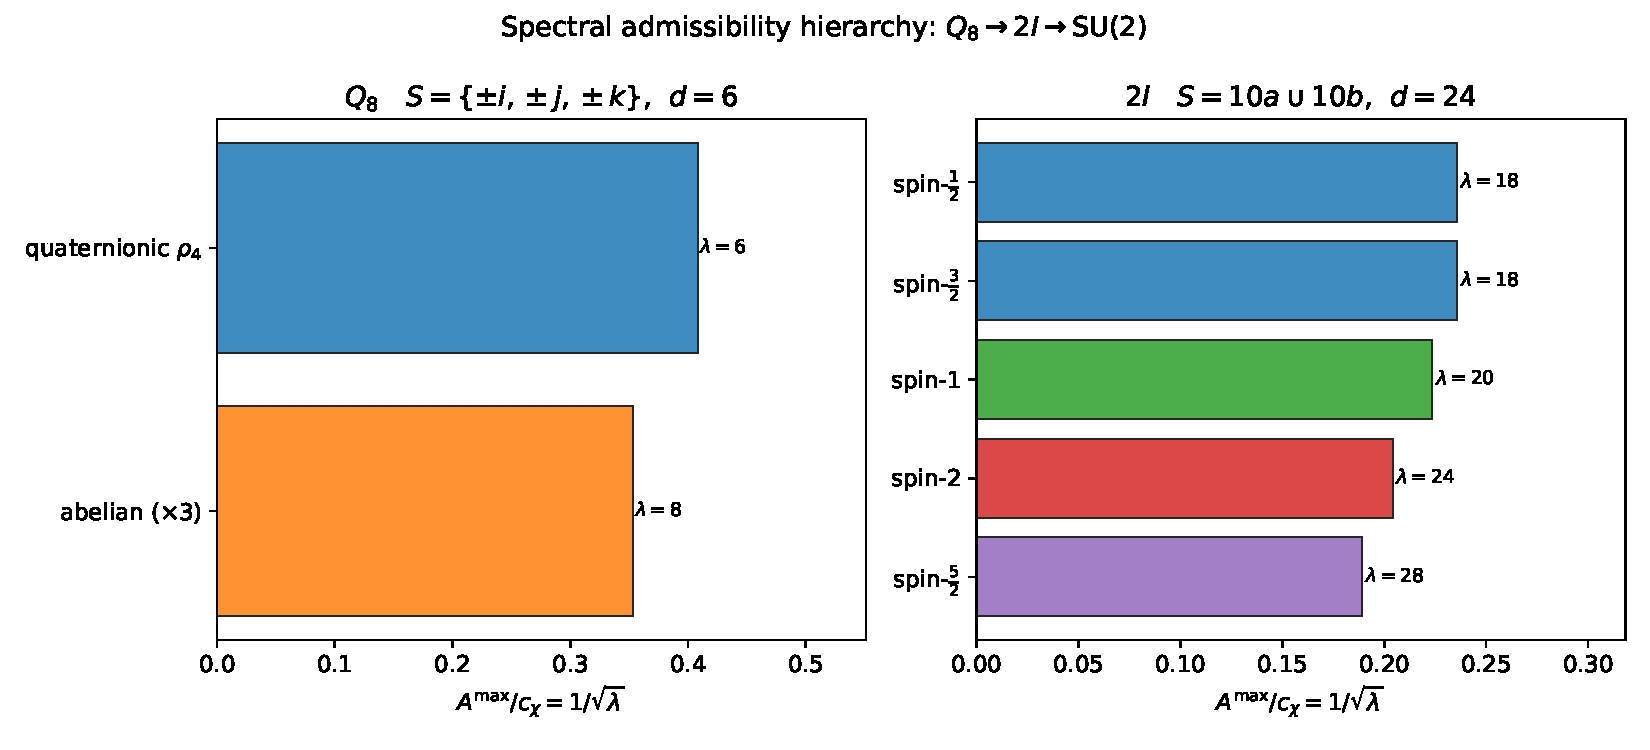
\includegraphics[width=0.95\textwidth]{fig3_hierarchy_Q8_vs_2I}
      \caption{
        Spectral admissibility hierarchy from $Q_8$ to $2I$.
        Left: on $Q_8$, the quaternionic sector has the smallest non-trivial
        Laplacian eigenvalue.
        Right: on $2I$ with generating set $S=10a\cup 10b$, the hierarchy
        resolves into the ordered spin-type sectors
        $\lambda_{1/2}=\lambda_{3/2}=18 < \lambda_1=20 < \lambda_2=24 <
        \lambda_{5/2}=28$.
        The comparison illustrates the sharpening of the admissibility
        hierarchy along the chain $Q_8 \subset 2I \subset \mathrm{SU}(2)$.
      }
      \label{fig:q8-2i-hierarchy}
    \end{figure}

    On $Q_8$ with $S=\{\pm i,\pm j,\pm k\}$,
    \begin{equation}
      \frac{A^{\max}_{\mathrm{best}}}{A^{\max}_{\mathrm{worst}}}
      = \sqrt{\frac{8}{6}}
      = \sqrt{\frac{4}{3}}
      \approx 1.155.
      \label{eq:Q8-ratio}
    \end{equation}

    On $2I$ with $S = 10a \cup 10b$, the corresponding ratio is
    \begin{equation}
      \frac{A^{\max}_{1/2}}{A^{\max}_{5/2}}
      = \sqrt{\frac{28}{18}}
      = \sqrt{\frac{14}{9}}
      \approx 1.247.
      \label{eq:2I-ratio}
    \end{equation}

    Thus the admissibility contrast increases from $Q_8$ to $2I$:
    \begin{equation}
      \sqrt{\frac{4}{3}}
      \approx 1.155
      \quad\longrightarrow\quad
      \sqrt{\frac{14}{9}}
      \approx 1.247.
      \label{eq:growing-hierarchy}
    \end{equation}

  \subsection{Physical interpretation: towards low-spin selection}
    \label{sec:step5-physics}

    On $Q_8$, the admissibility hierarchy separated the non-abelian sector from
    the abelian sectors.
    On $2I$, the hierarchy is resolved across several spin sectors:
    \begin{equation}
      \text{spin-}\tfrac{1}{2},\,\text{spin-}\tfrac{3}{2}
      \;\succ\;
      \text{spin-}1
      \;\succ\;
      \text{spin-}2
      \;\succ\;
      \text{spin-}\tfrac{5}{2},
      \label{eq:spin-ladder}
    \end{equation}
    where $\succ$ denotes a strictly larger admissibility window.

    The ordering is not strictly monotone in spin, since the
    spin-$\tfrac{1}{2}$ and spin-$\tfrac{3}{2}$ sectors are degenerate.
    Even so, the hierarchy is clearly biased toward lower spins.

  \section{Next Steps}
  \label{sec:next}

  The programme has now established spectral admissibility on two finite
  subgroups of $\mathrm{SU}(2)$:
  \begin{center}
    \renewcommand{\arraystretch}{1.2}
    \begin{tabular}{lll}
      \hline
      Step & Group & Key result \\
      \hline
      1--3 & $Q_8$ & $\lambda_{\text{non-ab}} = 6 < \lambda_{\text{abel}} = 8$;
      admissibility ratio $\sqrt{4/3}$ \\
      4 & $Q_8$ & structural origin via Pauli tracelessness
      ($\mu_{\rho_4} = 0$) \\
      5 & $2I$ & four-level hierarchy; ratio $\sqrt{14/9}$;
      origin via $\varphi - 1/\varphi = 1$ \\
      \hline
    \end{tabular}
  \end{center}

  Both results are exact, non-perturbative, and derived from character
  theory alone.
  The hierarchy strengthens along the inclusion chain
  $Q_8 \subset 2I \subset \mathrm{SU}(2)$, and its algebraic origin is
  structural at each step.

  \paragraph{Step~6: Large Cayley graphs approaching $\mathrm{SU}(2)$.}

    The natural continuation is to test whether the spectral hierarchy
    persists and sharpens along a family of Cayley graphs whose size grows
    without bound while the geometry converges toward
    $\mathrm{SU}(2) \cong S^3$.
    The complete programme chain is
    \begin{equation}
      Q_8
      \;\longrightarrow\;
      2I
      \;\longrightarrow\;
      \mathrm{SL}(2,\mathbb{F}_p)
      \;\xrightarrow{\;p \to \infty\;}
      \mathrm{SU}(2),
      \label{eq:chain-full}
    \end{equation}
    where the final arrow denotes local spectral convergence of the Cayley
    graphs toward the $S^3$ Laplacian.

    Natural candidates are the Ramanujan graphs of Lubotzky, Phillips, and
    Sarnak~\cite{LPS1988} on $\mathrm{SL}(2,\mathbb{F}_p)$.
    These graphs have three properties that make them ideal for the
    programme:

    \begin{enumerate}
      \item \emph{Near-optimal spectral gap.}
      The non-trivial Laplacian eigenvalues satisfy
      $\lambda \ge d - 2\sqrt{d-1}$ (Alon--Boppana bound),
      where $d = p + 1 = |S|$.
      The admissibility envelope
      $A^{\max}_\rho = c_\chi/\sqrt{\lambda_\rho}$ therefore remains
      uniformly controlled as $p$ grows.

      \item \emph{Increasing size.}
      $|\mathrm{SL}(2,\mathbb{F}_p)| = p(p^2-1)$ provides a sequence of
      progressively finer discrete approximations to $S^3$.

      \item \emph{Full spin tower in the limit.}
      The irreducible representations of $\mathrm{SL}(2,\mathbb{F}_p)$
      include all half-integer spins
      $j = 0, \tfrac12, \ldots, \tfrac{p-1}{2}$,
      reproducing the complete spin spectrum of $\mathrm{SU}(2)$ as
      $p \to \infty$.
    \end{enumerate}

    Step~6 consists of four sub-tasks.

    \medskip
    \noindent\textbf{Step~6a (generating set).}
    The LPS construction provides an explicit symmetric set of $p+1$
    generators of $\mathrm{SL}(2,\mathbb{F}_p)$, defined by the solutions to
    $a^2+b^2+c^2+d^2 \equiv 1 \pmod p$ with $a$ odd and $b,c,d$ even,
    embedded via the standard quaternion-to-matrix map.
    This set plays the same structural role as the generators
    $\{\pm i,\pm j,\pm k\}$ of $Q_8$ and the order-10 elements of $2I$.

    \medskip
    \noindent\textbf{Step~6b (character computation).}
    For any Cayley graph generated by a union of conjugacy classes,
    the adjacency eigenvalue in the irreducible sector $\rho$ is
    \begin{equation}
      \mu_\rho
      =
      \frac{1}{\dim\rho}
      \sum_{C \subseteq S} |C|\,\chi_\rho(C).
      \label{eq:mu-SL2}
    \end{equation}
    The character tables of $\mathrm{SL}(2,\mathbb{F}_p)$ are classical,
    and the spin-$j$ sector corresponds to the representation
    $\mathrm{Sym}^{2j}(V_2)$, exactly as in the $Q_8$ and $2I$ cases.

    \medskip
    \noindent\textbf{Step~6c (admissibility envelope).}
    The Laplacian eigenvalue and admissibility window for the spin-$j$
    sector are
    \begin{equation}
      \lambda_j = (p+1) - \mu_j,
      \qquad
      A^{\max}_j = \frac{c_\chi}{\sqrt{\lambda_j}}.
      \label{eq:Amax-SL2}
    \end{equation}

    \medskip
    \noindent\textbf{Step~6d ($p\to\infty$ limit).}
    The key observable is the ratio
    \begin{equation}
      R_p
      =
      \frac{A^{\max}_{j=1/2}}{A^{\max}_{j=j_{\max}}}
      =
      \sqrt{\frac{\lambda_{j_{\max}}}{\lambda_{1/2}}},
      \qquad
      j_{\max} = \frac{p-1}{2}.
      \label{eq:ratio-p}
    \end{equation}

    The programme predicts $R_p>1$ for all finite $p$,
    meaning that the spin-$\tfrac12$ sector remains the most
    admissible sector along the sequence.

    If the ordering
    $\lambda_{1/2} < \lambda_1 < \cdots < \lambda_{j_{\max}}$
    becomes monotone for large $p$ and
    $\lim_{p\to\infty} R_p > 1$,
    this would establish
    \begin{equation}
      \text{bounded relational flux}
      \;\Longrightarrow\;
      \text{monotone low-spin survival}
      \quad
      \text{in the }\mathrm{SU}(2)\text{ limit.}
      \label{eq:conclusion}
    \end{equation}

    The results on $Q_8$ and $2I$ already provide the first two
    non-trivial instances of this mechanism.
    Their algebraic origins — Pauli tracelessness and the golden-ratio
    identity $\varphi - 1/\varphi = 1$ — are both instances of the same
    underlying principle: the generating set $S$ is positively correlated
    with the low-spin representations in character.
    This yields
    $\mu_{\text{low spin}} > \mu_{\text{high spin}}$
    and therefore
    $\lambda_{\text{low}} < \lambda_{\text{high}}$.

    Whether this structural correlation persists uniformly along the chain
    \eqref{eq:chain-full} is the central open question of Step~6.

\end{document}
